\documentclass{article}
\linespread{0.7}
\usepackage[a4paper, margin=3mm, landscape]{geometry}
\usepackage{multicol}
\usepackage{xcolor}
\usepackage{enumitem}
\usepackage{amsmath}
\usepackage{amsfonts}
\usepackage{listings}
\usepackage{soul}
\usepackage{graphicx}

\pdfinfo{
    /Title (ee3801-cheatsheet.pdf)
    /Creator (TeX)
    /Producer (pdfTeX 1.40.0)
    /Author (Vincent Pang)
    /Subject (template)
    /Keywords (cheatsheet, pdf, ee3801)
}

\graphicspath{ {./img/} }

\pagestyle{empty}
\setcounter{secnumdepth}{0}
\setlength{\columnseprule}{0.25pt}

% Redefine section commands to use less space
\makeatletter
\renewcommand{\section}{\@startsection{section}{1}{0mm}%
    {-1ex plus -.5ex minus -.2ex}%
    {0.5ex plus .2ex}%x
{\normalfont\large\bfseries}}
\renewcommand{\subsection}{\@startsection{subsection}{2}{0mm}%
    {-1explus -.5ex minus -.2ex}%
    {0.5ex plus .2ex}%
{\normalfont\normalsize\bfseries}}
\renewcommand{\subsubsection}{\@startsection{subsubsection}{3}{0mm}%
    {-1ex plus -.5ex minus -.2ex}%
    {1ex plus .2ex}%
{\normalfont\small\bfseries}}%
\makeatother

% Adjust spacing for all itemize/enumerate
\setlength{\leftmargini}{0.5cm}
\setlength{\leftmarginii}{0.5cm}
\setlist[itemize,1]{leftmargin=2mm,labelindent=1mm,labelsep=1mm}
\setlist[itemize,2]{leftmargin=2mm,labelindent=1mm,labelsep=1mm}

% Font
\renewcommand{\familydefault}{\sfdefault}

% Define colors for math formulas
\definecolor{myblue}{cmyk}{1,.72,0,.38}
\everymath\expandafter{\the\everymath \color{myblue}}

% Custom command for keywords
\definecolor{highlight}{RGB}{251,243,218}
\newcommand{\keyword}[2][]{\sethlcolor{highlight}\hl{\textbf{#2}} #1 - }
\newcommand{\ilkeyword}[1]{\sethlcolor{highlight}\hl{\textbf{#1}}}

% Define colors and style for code
\definecolor{codegreen}{rgb}{0,0.6,0}
\definecolor{codegray}{rgb}{0.5,0.5,0.5}
\definecolor{codered}{HTML}{CC241D}
\definecolor{backcolor}{rgb}{0.95,0.95,0.95}
\lstdefinestyle{codestyle}{
    backgroundcolor = \color{backcolor},
    commentstyle = \color{codegray},
    keywordstyle = \color{codered},
    stringstyle = \color{codegreen},
    basicstyle = \ttfamily,
    breakatwhitespace = false,
    showstringspaces = false,
    breaklines = true,
    showtabs = false,
    tabsize = 2
}
\lstset{style = codestyle}

% -----------------------------------------------------------------------
\begin{document}
\begin{multicols*}{3}
\footnotesize

% Title box
\begin{center}
    \fbox{
        \parbox{0.8\linewidth}{
            \centering \textcolor{black}{
                {\Large\textbf{EE3801 Cheatsheet}} \\
                \normalsize{Intro to Data Engineering}} \\
                {\footnotesize \textcolor{gray}{github.com/securespider}}
        }
    }
\end{center}
\section{01.1 Intro}
\subsection{Data science vs engineering}
\begin{itemize}
	\item \keyword{Science}{Learn, optimise, analytics, aggregate and labelling}
	\item \keyword{Engineering}{Cleaning, data storage, logging, sensors, pipelines}
\end{itemize}
\subsection{Data structure}
\subsubsection{Unstructured data}
\begin{itemize}
	\item{Chaotic no order to data}
\end{itemize}
\subsubsection{Structured data}
\begin{itemize}
	\item Data stored access in the same format
\end{itemize}
\subsubsection{Semi structured data}
\begin{itemize}
	\item Can contain both forms of data 
	\item Some structure but not all data points follow same format
\end{itemize}
\subsection{Big data}
\begin{description}
	\item[Volume, Variety, Variability]
	\item[Velocity]{High rate of data generation}
	\begin{itemize}
		\item Must create a robust and scalable pipeline
	\end{itemize}
\end{description}
\subsection{Raw Data}
\begin{itemize}
	\item Tend to have gaps
\end{itemize}
\subsubsection{Data wrangling}
Used to understand raw data
\begin{description}
	\item[Discovery]{Understand what is in your data}
	\item[Structure]
	\item[Cleaning]{Dealing with gaps (nulls), outliers, formatting bugs}
	\item[Enrichment]{Derive other data from other information/ additional data augmentation (feature selection)}
	\item[Validation]{Verify data quality, sources}
	\item[Publishing]{Give data scientist}
\end{description}
\subsection{Process}
\begin{description}
	\item[Extraction]{Retrieve raw data from unstructured pool and migrate to temp repo}
	\item[Transformation]{Structure enrich and convert raw data}
	\item[Loading]{Loading structured data into data warehouse}
\end{description}
\subsubsection{Data warehouse}
Decision support system storing historical data from organisations
\subsubsection{Data Pipeline}
\begin{itemize}
	\item Processing underlying raw data in ordered sequence of steps
\end{itemize}

\section{01.2 Data Pipelines}
\subsection{Considerations}
\subsubsection{Big data}
\begin{description}
	\item[Velocity]{Streaming, captured and processed in real time}
	\item[Volume]{Scalable wrt time}
	\item[Variety]{Recognise and process diff formats}
\end{description}
\subsubsection{Business}
\begin{itemize}
	\item Handling streaming data?
	\item How much data to expect (Time horizon/how much storage consumed)
	\item What type/how much processing in DP
	\item Where is data source? Need micro-services?
\end{itemize}
\subsection{Architecture}
\subsubsection{Batch-based DP}
\begin{itemize}
	\item Analysis of data that has been stored over a period of time
	\item $N$ independent tasks to process with $k$ stages
	\item Each stage takes max of $T$ time process input
	\item Diff stage can operate concurrently
	\item $t(N,k) = T\times(N+k-1)$
\end{itemize}
\subsubsection{Streaming-based DP}
\begin{itemize}
	\item Processing as data flows through system
	\item Logging and persistent result storage
\end{itemize}
\subsubsection{Lambda Architecture}
\begin{itemize}
	\item Combination of batch and streaming
	\item Separate processing engine for "batch" and "speed" layers combining in "service" layer
	\item Accounts for real-time streaming and historical batch analysis
	\item Encourage raw data storage and create new dst for queries
	\item Min errors for both layers reliably at fast speeds
\end{itemize}
\subsubsection{Kappa Architecture}
\begin{itemize}
	\item Replay data and process both layers in same single stream processing engine
	\item Good for big data architecture with cheaper hardware and focus on stream
\end{itemize}
\subsection{Design}
\begin{enumerate}
	\item Identify application and decide if DP needed
	\item Identify DP category (architecture)
	\item Understand working mechanism, parameters/variables
\end{enumerate}
\section{04. Big Data Computing Technology Platform}
\begin{itemize}
	\item Collection of interconnected stand-alone computers
	\item Work collectively and cooperatively as an integrated computing resource pool
	\begin{itemize}
		\item Clusters exploit massive parallelism at job level
		\item Achieves high availability through stand-alone operations
		\item \keyword{Fault tolerance}{If one goes down, other can take over}
	\end{itemize}
\end{itemize}
\subsubsection{Benefits}
\begin{itemize}
	\item Scalable performance, high availability, fault tolerance
	\item Modular growth and use of commodity components
\end{itemize}
\subsubsection{Beowulf Cluster}
\begin{itemize}
	\item Single compute job requires frequent communication among cluster nodes
	\item Cluster share dedicated network
	\item Nodes are homogeneous and coupled
	\item eg. Each process requires information from other process
\end{itemize}
\subsection{Scalability}
Limited by:
\begin{itemize}
	\item Multicore chip technology, cluster topology, packaging method, power consumption and cooling scheme
	\item Memory capacity, disk IO bottlenecks, latency tolerance
\end{itemize}
\subsection{Packaging}
\begin{description}
	\item[Compact]{Nodes closely packaged in racks where nodes are not attached to peripherals}
	\item[Slack]{Nodes attached to peripherals connected remotely}
\end{description}
\subsubsection{Interconnection Medium}
Considerations
\begin{enumerate}
	\item Available link speeds
	\item Message Passing Interface (MPI) latency
	\item Network processor/routing mechanism/flow control
	\item Differing network topologies
\end{enumerate}
\textbf{Self routing/Destination tag} \\
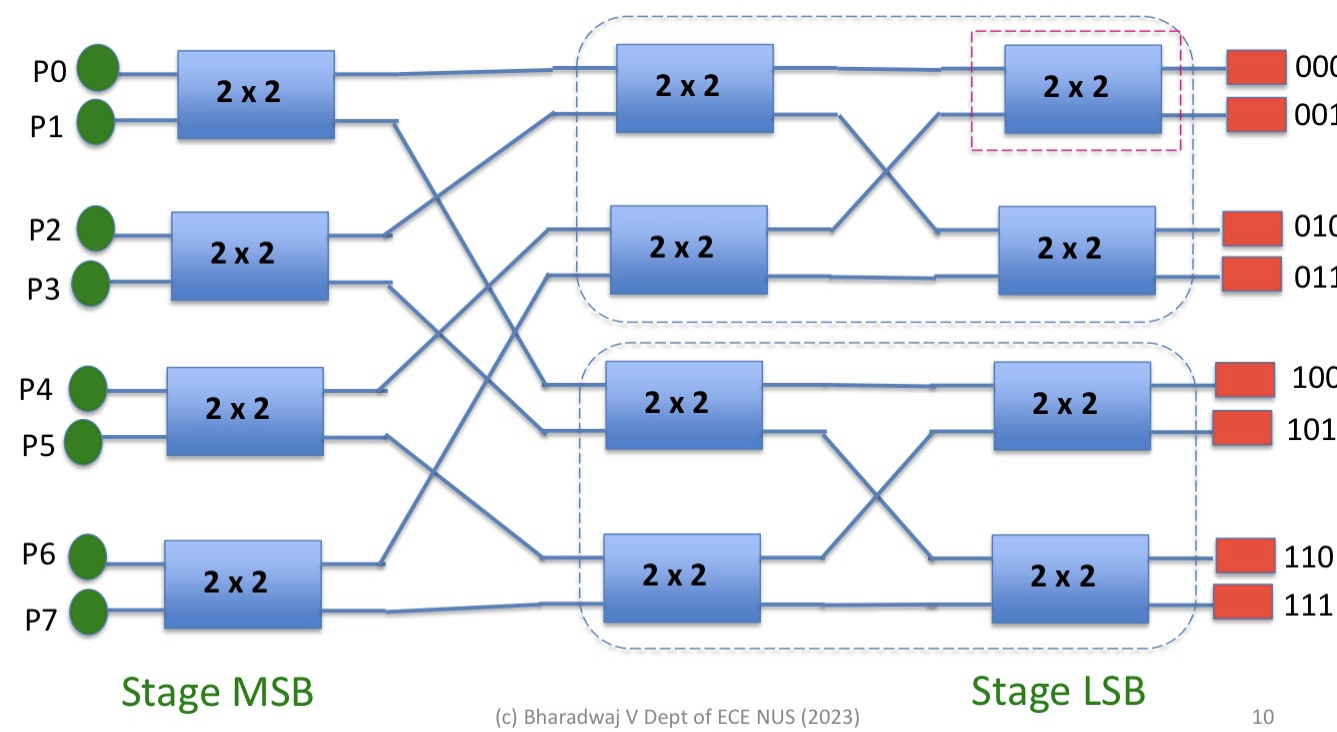
\includegraphics[scale=0.2]{self-routing}
\begin{itemize}
	\item Every processor can be routed to every memory without external controller
	\item Switch should know what stage it is in to know which bit to look for
	\item Bit of stage defines which output interface it leaves (0-above, 1-below)
\end{itemize}
\subsection{Control}
\begin{description}
	\item[Centralized]{Nodes owned, ctrl by central operator}
	\begin{itemize}
		\item Easy to manage 
		\item Used by compact and slack clusters
	\end{itemize}
	\item[Decentralized]{Nodes have individual owners}
	\begin{itemize}
		\item Minimize coupling and can be used w many OS
		\item Only slack can have
	\end{itemize}
\end{description}
\subsubsection{Homogeneity}
\begin{description}
	\item[Homogeneous]{Nodes from same platform (architecture and operating system)}
	\item[Heterogeneous]{Nodes of different platforms and different operating systems}
	\begin{itemize}
		\item Can run and share with everyone 
	\end{itemize}
\end{description}
\subsection{Programmability}
\begin{itemize}
	\item Cluster Operating System (COS) must provide user friendly interface btw user, application and hardware
	\item Additional features like single-system image and system availability
	\item Ensure failure management, load balancing and tools for parallelizing computation
\end{itemize}
\subsubsection{COS Examples}
\begin{description}
	\item[Solaris MC]{Prototype, distributed operating system for multi-computers}
	\item[MOSIX]{Software package that extends the Linux1 kernel with cluster computing capabilities}
	\begin{itemize}
		\item Allows any size cluster of Intel-based computers to work together like single system like SMP (Symmetrical Multi Processor)
	\end{itemize}
	\item[GLUnix]{Global Layer Unix - Global operating system for Berkeley's Network of Workstations (NOW)}
	\begin{itemize}
		\item NOW's goal was to construct a platform that would support both parallel and sequential applications on commodity hardware
		\item Has load balancing capability
	\end{itemize}
\end{description}
\subsubsection{Window-based Load Balancing technique}
\begin{enumerate}
	\item Core node C broadcast REQ msg to all nodes for status collection
	\item Each node sends current load info to C 
	\item C computes average load and deficit/surplus for each node
	\item C sends MIGRATION msg to each node to transfer excess to deficit nodes
	\item After some time $w$, after migration, C repeats process
\end{enumerate}
\begin{itemize}
	\item Centralised controlled by core node
	\item $w$ impt to decide as 
	\begin{enumerate}
		\item Communication overhead with frequent trf
		\item C may be working with outdated info
	\end{enumerate}
\end{itemize}
\subsection{Security}
\begin{itemize}
	\item Intra-cluster communication can be \textbf{exposed/enclosed}
\end{itemize}
\begin{description}
	\item[Exposed cluster]{Communication paths among the nodes exposed to outside world}
	\begin{itemize}
		\item Using standard protocols eg. TCP/IP
		\item ICC need effort to ensure privacy and security
		\item Outside communications may disrupt ICC in unpredictable fashion
		\item May have high overhead 
	\end{itemize}
	\item[Enclosed]{Shielded from outside world}
	\begin{itemize}
		\item No standard for efficient enclosed ICC
	\end{itemize}
\end{description}
\subsection{Resource sharing}
\begin{itemize}
	\item Clustering improves both availability and performance
	\item High Availability clusters use hardware redundancy for scalable performance
	\item All connects to NIC component in node
\end{itemize}
\begin{description}
	\item[Share-nothing]{Each node do itself and send results together after}
	\begin{itemize}
		\item Simple to configure and used in most clusters
		\item Nodes connected through I/O bus eg Ethernet
	\end{itemize}
	\item[Shared-disk]{When one node fail the other take over}
	\begin{itemize}
		\item Used in small-scale availability clusters in business applications
		\item Fault tolerance via checkpoints, rollback, failover..
	\end{itemize}
	\item[Shared-memory]{All common data/instruction written in shared space}
	\begin{itemize}
		\item Nodes connected by Scalable Coherence Interface (SCI) ring which is connected to memory bus of each node through NIC module
		\item Memory bus operated at higher frequency than the I/O bus
	\end{itemize}
\end{description}
\subsection{Cloud Computing Platforms}
\begin{itemize}
	\item Cluster and Grid computing leverage use of many computers in parallel to solve problems of any size
	\item Utility and Software as a Service provide computing resources as a service (pay per use)
	\item Utility/Cloud computing - High throughput computing paradigm 
	\begin{itemize}
		\item Provides services through large data center or distributed server farms
		\item Leverage dynamic resources to deliver large number of services to end users
		\item Enables users to share access to resources from anywhere with connected devices
		\item Frees low-level tasks of setting up hardware 
		\item Manage system software at low cost and easy-to-use manner
		\item Applies virtual platform with "elastic resources"
		\item Comprise of Core Layer $\leftrightarrow$ Aggregate Layer $\leftrightarrow$ Access layer $\leftrightarrow$ Leaf nodes
	\end{itemize}
\end{itemize}
\subsection{Accessibility}
\begin{itemize}
	\item Compute probability of successful access to the cloud
	\item Data Center (DC) comprise cloud layers + core, aggregate, access layers and leaf nodes in hierarchical system
\end{itemize}
\subsection{Cloud vs Data Center}
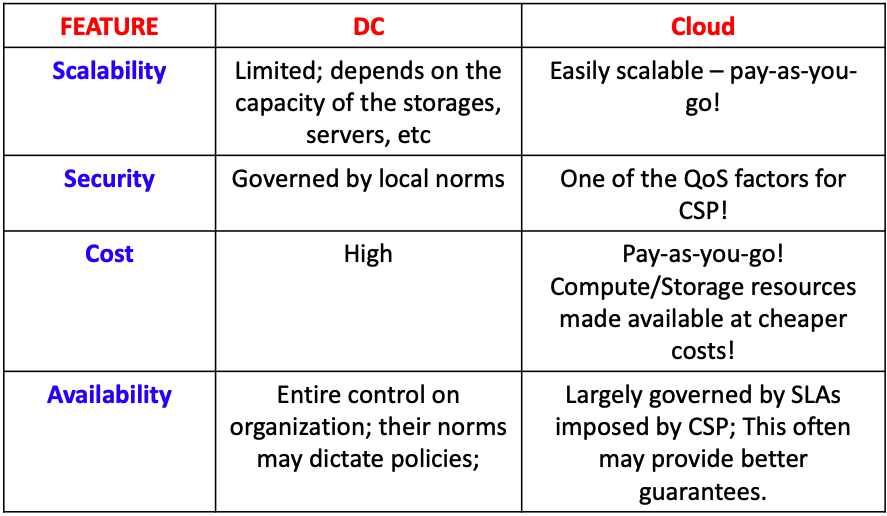
\includegraphics[scale=0.2]{4_1-cloud-vs-dc}
\subsection{Virtualization}
\begin{itemize}
	\item Computer file/Image that behaves like an actual computer
	\item VM runs in a separate window like a program giving end user an identical experience as on host system
	\item VM is sandboxed from rest of system
	\begin{itemize}
		\item Risky operations eg testing operating system or malwares 
		\item Running software on different OS/ OS backups
	\end{itemize}
\end{itemize}
\subsubsection{Implementation}
\begin{itemize}
	\item Hypervisor installed on physical hardware used to create and amange VMs 
	\item Each VM has virtual computing resources and can run simultaneously
	\item Multiple OS run side by side using hypervisors to manage
\end{itemize}
\section{4.2 Big Data Computing Technology}
\begin{itemize}
	\item Platforms and Cloud Security - On Cloud
	\item Data Security and Storage
	\begin{itemize}
		\item Security and privacy in cloud platforms
		\item Data security - components and issues
		\item Data Integrity, Confidentiality, Availability, Privacy
		\item Commonly used data encryption algorithms in Cloud
		\item Distributed Data Storage
	\end{itemize}
\end{itemize}
\subsection{Service Models in Cloud Platforms}
\begin{description}
	\item[Software as a Service (SaaS)]{Software with related data deployed by Cloud Service Provider (CSP) that users can use through web browsers}
	\item[Platform as a service]{CSP facilitates service to the users by providing certain cloud components to certain software that can solve specific tasks}
	\item[Infrastructure as a Service]{CSP facilitates services to the users with virtual machines and storage to improve business capabilities}
\end{description}
\subsection{Cloud Categories}
\begin{description}
	\item[Public clouds]{Owned and operated by third-party CSP and delivered over the internet}
	\begin{itemize}
		\item Low-cost and scalability (pay-as-use)
		\item High reliability
		\item No maintenance on User's side
	\end{itemize}
	\item[Private]{Computing and Storage resources used exclusively by one specific business/organisation}
	\begin{itemize}
		\item These can be physically located at organisation's on-site DC or hosted by third-party
		\item All equipment and resource deployment depend on local policies and norms
		\item Scalability (but may not be low-cost)
		\item Highly secured storage and access
		\item Custom-driven local environments can be created as per the needs of the organisation
	\end{itemize}
	\item[Hybrid]{Combination of public/private}
	\begin{itemize}
		\item Take advantage of secured on premise infrastructure while using public cloud service
		\item Use public cloud feature for high-volume data handling
		\item Commonly used w lower security needs - web based email/web-page hosting
	\end{itemize}
\end{description}
\subsection{Security and privacy in cloud platform}
\begin{itemize}
	\item Combination of data integrity, confidentiality, availability and privacy
	\item Prevention of unauthorized disclosure, witholding, amendment or deletion of information
\end{itemize}
\subsubsection{Data Integrity}
\begin{itemize}
	\item Protecting data from unauthorized deletion, modification or fabrication
	\item Manage entity's admittance and rights to specific enterprise resources 
	\item Ensure valuable data and services are not abused misappropriated or stolen
\end{itemize}
\textbf{Data storage - Databases}
\begin{itemize}
	\item Easily achieved in a standalone system with single database
	\item Maintained via database constraints, transactions that follow ACID properties
	\begin{description}
		\item[Atomicity]{All operations are treated as atomic/single}
		\begin{itemize}
			\item Failure of transaction will restart/rollback to earlier saved state
		\end{itemize}
		\item[Consistency]{Mechanism that enforce rules across all nodes storing data}
		\item[Isolation]{Manage concurrent access without affecting other nodes}
		\item[Durability]{Guarantees data is saved safely after transaction admist failures while updating}
		\begin{itemize}
			\item Data is locked until transaction is completed
			\item Results are first written into local transaction logs and written into entry after work done
		\end{itemize}
	\end{description}
	\item Important in datalakes and DWH
	\item Allows users to see consistent views of data even while new data modified in real-time
	\item Trust stored data
\end{itemize}
\textbf{How to achieve}
\begin{itemize}
	\item \keyword{RAID}{Array of stored disks}
	\item Avoid unauthorised access
	\item Monitoring mechanisms to have greater transparency on any altered data
\end{itemize}
\subsubsection{Data Confidentiality}
\begin{itemize}
	\item Facilitates storing users' private or confidential data in cloud
	\item Authentication and access control strategies
	\item No trust in CSP as cannot store sensitive data (insider attacks)
	\item CSP can have different subscription level for varying confidentiality
\end{itemize}
\textbf{Distributed Storage}
\begin{itemize}
	\item Store data in multiple clouds or databases
	\begin{itemize}
		\item Data divided into chunks, encrypted and stored in different databases
		\item Since each segment encrypted and separately distributed, enhanced security against different attack
	\end{itemize}
\end{itemize}
\subsubsection{Data Availability}
\begin{itemize}
	\item Ensure data can be recovered and verified by techniques rather than guarantee by CSP
	\item Quickly and efficiently locate data 
	\item If a node is attacked, we cannot use any direct links from a node that leads to attacked node
\end{itemize}
\subsubsection{T-coloring problem}
\begin{itemize}
	\item Color vertices of graph st no adjacent nodes have identical colors
	\item Find the minimum number of colors needed
\end{itemize}
\textbf{Solution}
\begin{itemize}
	\item Generate all possible coloring of nodes and backtrack by avoiding certain color possibilities
\end{itemize}
\subsubsection{Data Privacy}
\begin{itemize}
	\item Seclude information/sensitive data to prevent adversary from inferring user behavior by visit model
	\item Using oblivious ram(ORAM) technology
	\begin{itemize}
		\item Visit several copies of data to hide real visiting aims of users
	\end{itemize}
\end{itemize}
\end{multicols*}
\end{document}
